\documentclass[aspectratio=169]{beamer}


\usepackage{amssymb,amsmath}
\usepackage{graphicx}
\usepackage{url}
\usepackage{color}
\usepackage{relsize}	% For \smaller
\usepackage{url}			% For \url
\usepackage{epstopdf}	% Included EPS files automatically converted to PDF to include with pdflatex
\usepackage{pgfpages} % necessary for note options, used for npages too.
% \usepackage{multimedia} % for movies


%%% NOTE OPTIONS %%%%%%%%%%%%%%%%%%%%%%%%%%%%%%%%%%%%%%%%%%%%%%%%%%%%%%%%%%%%

%% NOTE DISPLAY:
%\setbeameroption{show notes} % NOTES AS SLIDES
%\setbeameroption{show notes on second screen = left} % NOTES WITH SLIDES
%\setbeameroption{show only notes} % ONLY NOTES

%\setbeamertemplate{note page}[plain] % Uncomment this for simpler notes

%%%%%%%%%%%%%%%%%%%%%%%%%%%%%%%%%%%%%%%%%%%%%%%%%%%%%%%%%%%%%%%%%%%%%%%%%%%%%
%For MindMaps
% \usepackage{tikz}%
% \usetikzlibrary{mindmap,trees,arrows}%

%%% Color Definitions %%%%%%%%%%%%%%%%%%%%%%%%%%%%%%%%%%%%%%%%%%%%%%%%%%%%%%%%%
%\definecolor{bordercol}{RGB}{40,40,40}
%\definecolor{headercol1}{RGB}{186,215,230}
%\definecolor{headercol2}{RGB}{80,80,80}
%\definecolor{headerfontcol}{RGB}{0,0,0}
%\definecolor{boxcolor}{RGB}{186,215,230}

%%% Save space in lists. Use this after the opening of the list %%%%%%%%%%%%%%%%
% \newcommand{\compresslist}{
% 	\setlength{\itemsep}{1pt}
% 	\setlength{\parskip}{0pt}
% 	\setlength{\parsep}{0pt}
%}

%\setbeameroption{show notes on top}

% You should run 'pdflatex' TWICE, because of TOC issues.

\mode<presentation>
{
  % A tip: pick a theme you like first, and THEN modify the color theme, and then add math content.
  % Warsaw is the theme selected by default in Beamer's installation sample files.

  %%%%%%%%%%%%%%%%%%%%%%%%%%%% THEME
  %\usetheme{AnnArbor}
  %\usetheme{Antibes}
  %\usetheme{Bergen}
  %\usetheme{Berkeley}		% bem bacana - menu esquerdo
  %\usetheme{Berlin}
  %\usetheme{Boadilla}
  %\usetheme{boxes}
  %\usetheme{CambridgeUS}		% bem bacana - menu superior
  %\usetheme{Copenhagen}                 % not good for multiple sections
  %\usetheme{Darmstadt}        % Same as frankfurt with subsection names
  %\usetheme{default}
  %\usetheme{Dresden}
  %\usetheme{Frankfurt}         % My ``standard''
  %\usetheme{Goettingen}
  %\usetheme{Hannover}		% bem bacana - menu esquerdo
  %\usetheme{Ilmenau}
  %\usetheme{JuanLesPins}
  %\usetheme{Luebeck}
  \usetheme{Madrid}		%bacana
  %\usetheme{Malmoe}
  %\usetheme{Marburg}		% bem bacana - menu direito
  %\usetheme{Montpellier}
  %\usetheme{PaloAlto}		% bem bacana - menu esquerdo
  %\usetheme{Pittsburgh}
  %\usetheme{Rochester}		%bacana
  %\usetheme{Singapore}
  %\usetheme{Szeged}
  %\usetheme{Warsaw}

  %%%%%%%%%%%%%%%%%%%%%%%%%%%% COLOR THEME
  %\usecolortheme{albatross}		% azul escuro, massa
  %\usecolortheme{beetle}		% cinza, menu azul
  %\usecolortheme{crane}		% branco e amarelo, massa
  %\usecolortheme{default}		% branco, azul clarinho
  \usecolortheme{dolphin}		% azul e branco, legal
  %\usecolortheme{dove}			% cinza e branco, feio
  %\usecolortheme{fly}			% todo cinza, horrível
  %\usecolortheme{lily}			% parece o default
  %\usecolortheme{orchid}		% azul e branco, ok
  %\usecolortheme{rose}			% branco e violeta-claro, bonito
  %\usecolortheme{seagull}		% cinza, feio
  %\usecolortheme{seahorse}		% nhé, meio feio
  %\usecolortheme{sidebartab}		% Azul, branco, destaque na tab, interessante
  %\usecolortheme{structure}		% bichado
  %\usecolortheme{whale}		% Azul e branco, bem bonito

  %%%%%%%%%%%%%%%%%%%%%%%%%%%% OUTER THEME
  % Theme for showing the section and sub section
  \useoutertheme{default}
  %\useoutertheme{infolines}
  %\useoutertheme{miniframes}
  %\useoutertheme{shadow}
  %\useoutertheme{sidebar}
  %\useoutertheme{smoothbars}
  %\useoutertheme{smoothtree}
  %\useoutertheme{split}
  %\useoutertheme{tree}

  %%%%%%%%%%%%%%%%%%%%%%%%%%%% INNER THEME
  %\useinnertheme{circles}
  \useinnertheme{default}
  %\useinnertheme{inmargin}
  %\useinnertheme{rectangles}
  %\useinnertheme{rounded}

  %%%%%%%%%%%%%%%%%%%%%%%%%%%%%%%%%%%

  \setbeamercovered{invisible} % or whatever (possibly just delete it)
  % To change behavior of \uncover from graying out to totally
  % invisible, can change \setbeamercovered to invisible instead of
  % transparent. apparently there are also 'dynamic' modes that make
  % the amount of graying depend on how long it'll take until the
  % thing is uncovered.

}


% Get rid of nav bar
\beamertemplatenavigationsymbolsempty

% Use short top
%\usepackage[headheight=12pt,footheight=12pt]{beamerthemeboxes}
%\addheadboxtemplate{\color{black}}{
%\hskip0.5cm
%\color{white}
%\insertshortauthor \ \ \ \
%\insertframenumber \ \ \ \ \ \ \
%\insertsection \ \ \ \ \ \ \ \ \ \ \ \ \ \ \ \ \  \insertsubsection
%\hskip0.5cm}
%\addheadboxtemplate{\color{black}}{
%\color{white}
%\ \ \ \
%\insertsection
%}
%\addheadboxtemplate{\color{black}}{
%\color{white}
%\ \ \ \
%\insertsubsection
%}

% Insert frame number at bottom of the page.
% \usefoottemplate{\hfil\tiny{\color{black!90}\insertframenumber}}



\usepackage[english]{babel}
%\usepackage[latin1]{inputenc}
\usepackage{subfigure}

\usepackage{times}
\usepackage[T1]{fontenc}

%%% Macro for putting images at arbitrary places
%% See http://tex.stackexchange.com/questions/34921/how-to-overlap-images-in-a-beamer-slide
\def\Put(#1,#2)#3{\leavevmode\makebox(0,0){\put(#1,#2){#3}}}

%%% Variable Block
%% See http://tex.stackexchange.com/questions/12550/changing-default-width-of-blocks-in-beamer
\newenvironment<>{varblock}[2][.9\textwidth]{%
  \setlength{\textwidth}{#1}
  \begin{actionenv}#3%
    \def\insertblocktitle{#2}%
    \par%
    \usebeamertemplate{block begin}}
  {\par%
    \usebeamertemplate{block end}%
  \end{actionenv}}


\usepackage{algorithm}
\usepackage{algpseudocode}

\title[Evolutionary Frankenstein]{Evolutionary Frankenstein:\\ From "metaphor algorithms" to "components research"}
\author[Claus Aranha]{Claus Aranha\\University of Tsukuba}
\date{2022-12-15}

\begin{document}

\section{Introduction}
\begin{frame}
  \maketitle

  \vfill

  \hfill\footnotesize{e-mail: caranha@cs.tsukuba.ac.jp}
\end{frame}


\begin{frame}{A little bit about myself}
  \begin{columns}
    \column{0.6\textwidth}
    \begin{itemize}
      \item Born in Brazil, living in Japan for a long time;
      \item Love programming:
      \begin{itemize}
        \item Recombine small words to make anything;
        \item Calculate, Visualize, Simulate;
        \item ... Games
        \item ... Art?
        \item ... Life???
      \end{itemize}
      \item Research: Artificial Evolution and Artificial Life;
      \item And also computer games;
    \end{itemize}
    \vfill
    \hfill ... Do crazy things with the computer!
    \column{0.4\textwidth}
    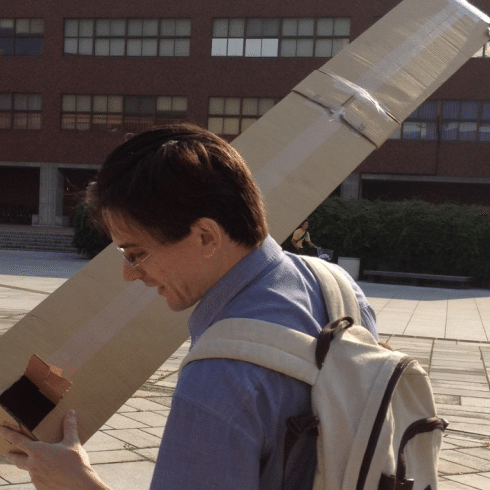
\includegraphics[width=.9\textwidth]{img/Claus_Eclipse}
  \end{columns}
\end{frame}

\begin{frame}{Outline of the Talk}

  {\bf Topic}: How to design algorithms that use \structure{Evolution} to solve optimization problems?\medskip

  {\bf Message}: It is possible ({\bf and fun!}) to create new techniques through \structure{careful study and recombination} of classic algorithms;\medskip

  {\bf Topics}:
  \begin{itemize}
    \item What is Evolutionary Computation?
    \item A few classic Evolutionary Computation algorithms;
    \item A LOT of weird algorithms; (and the problem with them);
    \item How can we keep the good and throw away the bad?
  \end{itemize}
\end{frame}

\section{Quick Guide to Evolutionary Computation}

\begin{frame}
  \begin{center}
  {\large{\bf
  Part I\\
  A quick guide to Evolutionary Computation
  }}
  \end{center}
\end{frame}

\subsection{What is Evolutionary Computation?}

\begin{frame}[t]{What is Evolutionary Computation?}
  \begin{columns}
    \column{0.7\textwidth}
    \begin{itemize}
      \item Natural Evolution is amazing:
      \begin{itemize}
        \item Creates a variety of incredible creatures;
        \item These creatures are \structure{well adapted} to their environment;
        \item \structure{Domain information} is not used {\bf a priori};
      \end{itemize}
      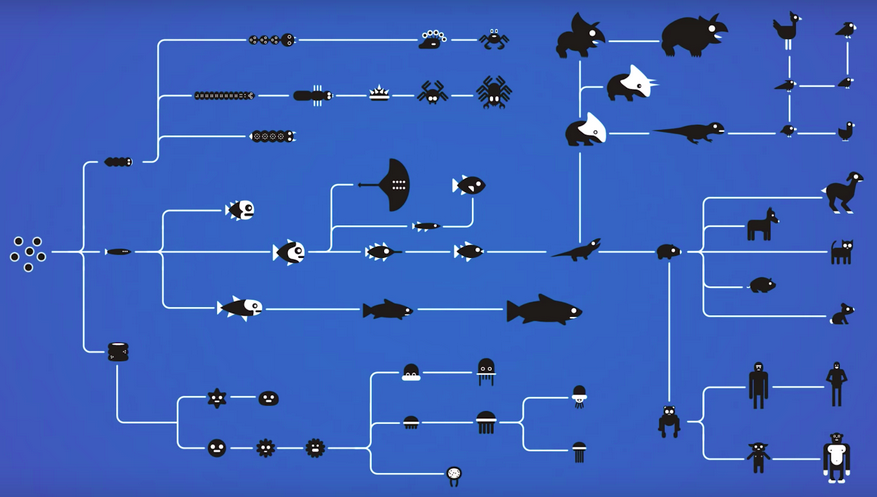
\includegraphics[width=0.7\textwidth]{img/OEE_Nature.png}

      \item Can we apply evolution to computational systems?
    \end{itemize}
    \column{0.3\textwidth}
    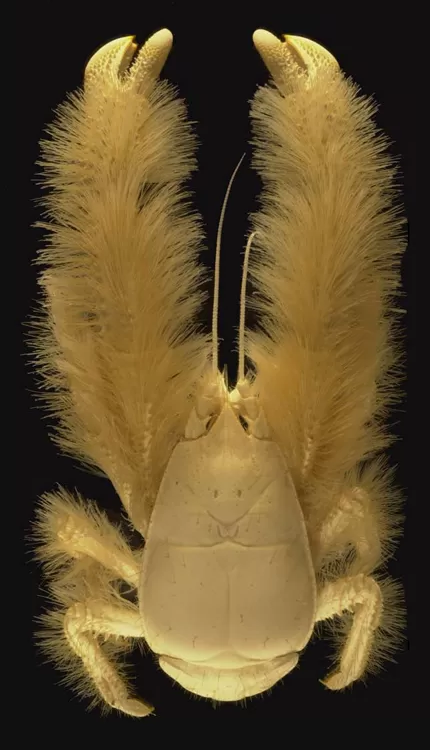
\includegraphics[width=0.9\textwidth]{img/underwater_3.png}
  \end{columns}
\end{frame}

\begin{frame}[t]{Evolutionary Computation is Cool}
  For over 50 years, researchers have developed an outline for  \structure{Artificial Evolution}:\bigskip

  \begin{itemize}
    \item Define the problem to be solved as {\bf The Environment}
    \item Define the solution to be found as {\bf The Individuals}
    \item Evaluate the individuals and give them a {\bf Fitness Score};
    \item Reproduce and Modify the individuals based on their Fitness;
  \end{itemize}
\medskip

This general algorithm has been used to solve many hard problems:

\hspace{0.2\textwidth}
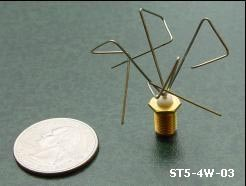
\includegraphics[height=0.4\textheight]{img/GA_Sattelite.png}
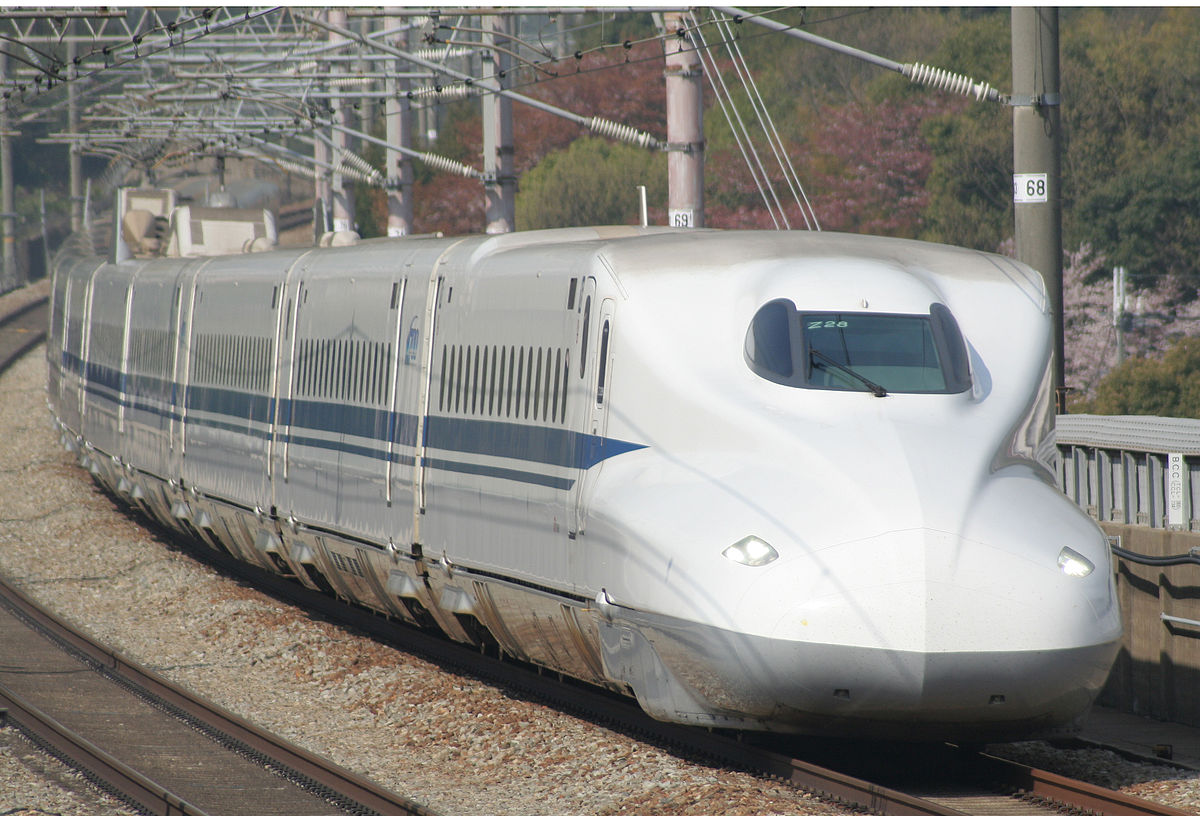
\includegraphics[height=0.4\textheight]{img/GA_N500.png}

\end{frame}

\begin{frame}{Why does Evolutionary Computation Work?}
  Evolutionary Computation is commonly applied to \structure{Optimization Problem}:
  \begin{quote}
  Find a vector $x \in \mathbb{R}^d$, that minimizes the value of $f(x)$
  \end{quote}\bigskip

  It works by testing several solutions, until it finds a solution that works. This is also called \structure{Search Based Optimization (SBO)}.

  \begin{itemize}
    \item SBO does not depend on gradient, so it works for discontinuous problems;
    \item SBO does not require domain knowledge, so it is a \emph{general} method;
  \end{itemize}\bigskip

  Also, algorithms based on Evolutionary Computation are \structure{very easy to implement}, and also easy to parallelize.\medskip

  Let's see some classical Evolutionary Computation algorithms.
\end{frame}




\subsection{Some Classical Evolutionary Optimizers}
% \begin{frame}{Simulated Annealing}{YY 19XX}
% % Note: Not exactly an evolutionary algorithm, but part of the family
% \end{frame}

\begin{frame}{Evolution Strategy (ES)}{Rechenberg and Schwefel, 1971}
  \begin{columns}
    \column{0.5\textwidth}
    \structure{Key idea}:
    Offspring with beneficial mutations replace the parent.\bigskip

    \begin{center}
      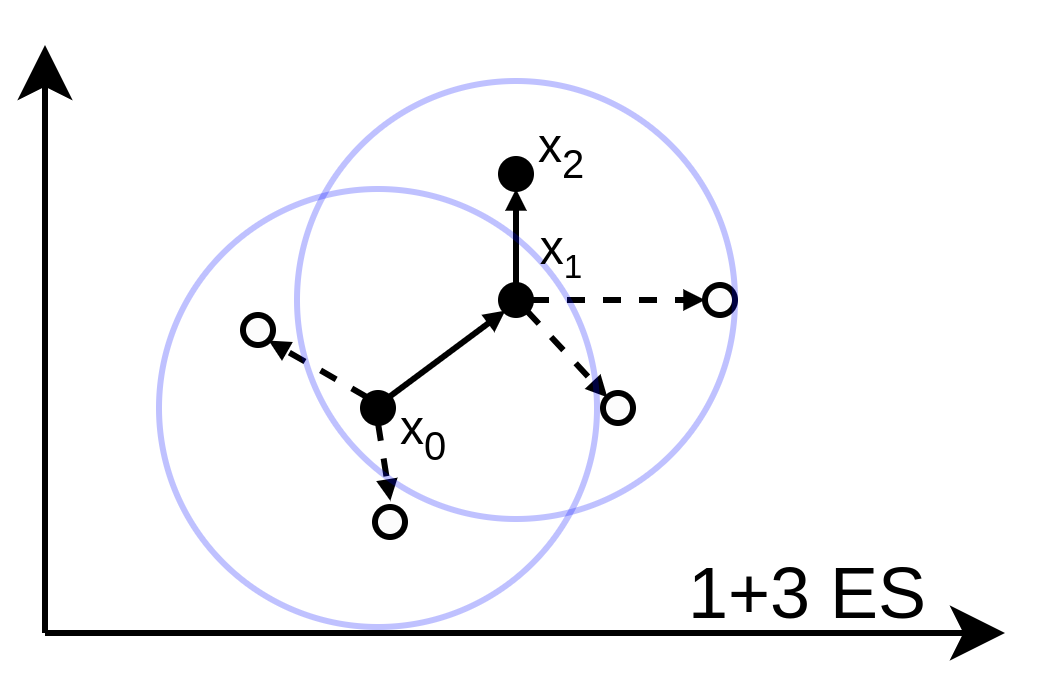
\includegraphics[width=0.7\textwidth]{img/ES_one_lambda.png}
    \end{center}

    Later versions adapt the mutation step $s$ during the optimization.


    \column{0.5\textwidth}
      Evolution Strategy (1+$\lambda$-ES)\bigskip

      \begin{algorithmic}[1]
        \Require $x \in \mathbb{R}^d$ (Initial Solution)
        \Require $\lambda$: number of offspring
        \Require $s$: step size
        \While{{\bf not} terminate condition}
          \For{$i: 0 \to \lambda$}
          \State $o_i \gets x + N(0,1)^d * s$
          \EndFor
          \State $o_b \gets$ best $o_i$
          \State {\bf If} $o_b$ {\bf better than} $x$: $x \gets o_b$
        \EndWhile
        \State {\bf Output $x$}
      \end{algorithmic}
  \end{columns}
\end{frame}

\begin{frame}{Genetic Algorithm}{Holland, 1975}
  \begin{columns}
    \column{0.5\textwidth}
    \structure{Key ideas}:
    \begin{itemize}
      \item Population tracks several solutions in parallel;
      \item Selection bias search to good solutions;
      \item Crossover exchanges building blocks;
    \end{itemize}

    \begin{center}
      \includegraphics[width=0.7\textwidth]{img/GA_crossover.png}
    \end{center}

    These three ideas imply that good building blocks spread through the population (\structure{schemata theory})

    \column{0.5\textwidth}
      Genetic Algorithm\bigskip

      \begin{algorithmic}[1]
        \Require Binary Representation of Solution
        \Require $P \in \{1, 0\}^{d\times p}$ (Initial Population)
        \While{{\bf not} terminate condition}
          \State Evaluate fitness of population, $f(P)$
          \For{$i: 0 \to p$}
          \State Select parents $x_a$,$x_b$ by fitness
          \State $o_i \gets$ crossover$(x_a, x_b)$
          \State $o_i \gets$ mutation$(o_i)$
          \State Insert $o_i$ in $P_{\text{new}}$
          \EndFor
          \State $P \gets P_{\text{new}}$
        \EndWhile
        \State {\bf Output} best $x \in P$
      \end{algorithmic}
  \end{columns}
\end{frame}

\begin{frame}{Differential Evolution}{Storn and price, 1997}
  \begin{columns}
    \column{0.5\textwidth}
    \structure{Key idea}: Mutation based on the difference of two random solutions means that the \structure{mutation step automatically adapts} to the size of the population.

    \begin{center}
      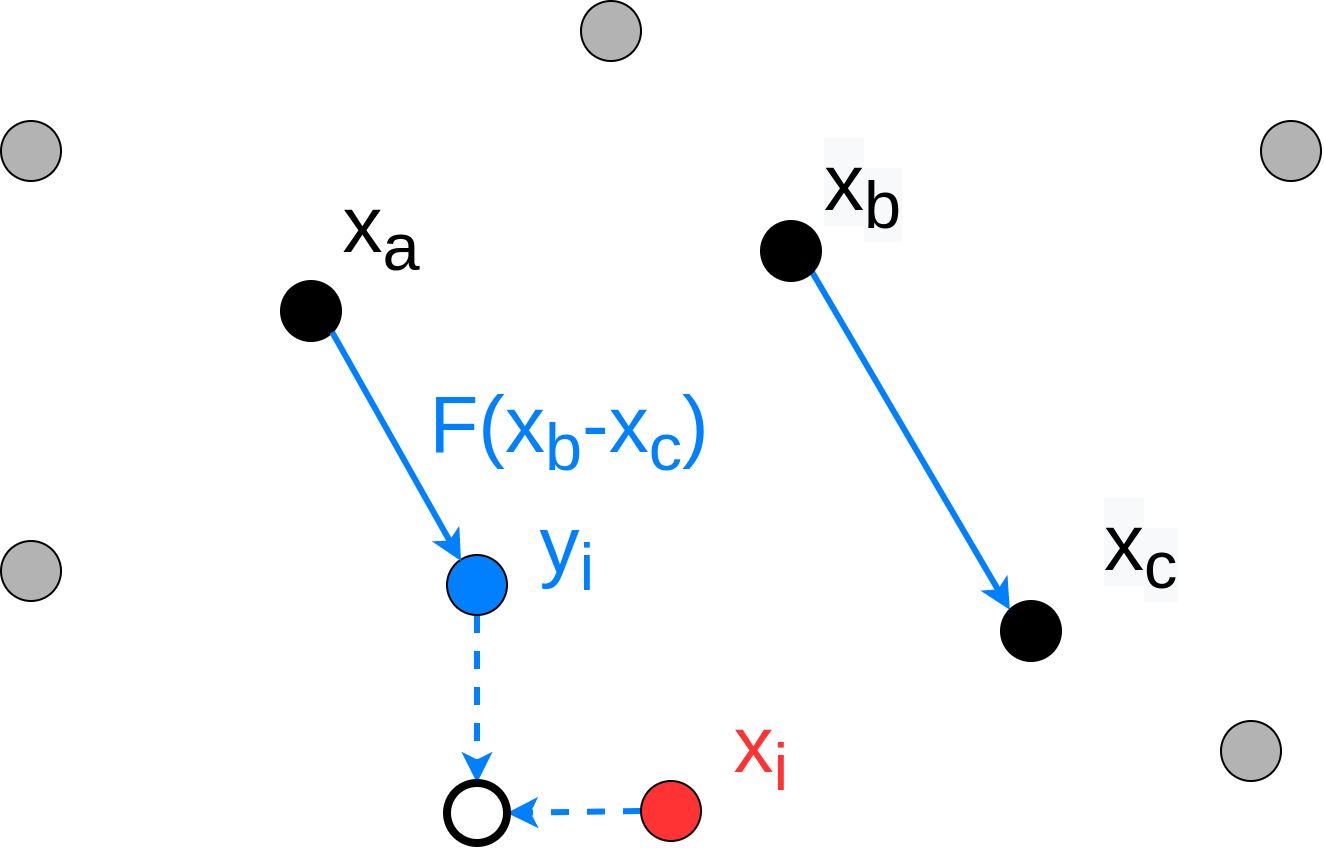
\includegraphics[width=0.7\textwidth]{img/DiffEvo.png}
    \end{center}

    \column{0.5\textwidth}
      Differential Evolution\bigskip

      \begin{algorithmic}[1]
        \Require $P \in \mathbb{R}^{d\times p}$ (Initial Population)
        \Require Parameters $F, Cr$
        \While{{\bf not} terminate condition}
          \For{$i: 0 \to p$}
          \State Choose random $x_a, x_b, x_c \in P$
          \State $y_i = x_a + F(x_b - x_c)$
          \For{$j: 0 \to d$}
          \State $y_{i,j} \gets x_{i,j}$ with prob $Cr$
          \EndFor
          \State {\bf If} $y_i$ better than $x_i$: $x_i \gets y_i$
          \EndFor
        \EndWhile
        \State {\bf Output} best $x \in P$
      \end{algorithmic}
  \end{columns}
\end{frame}

\begin{frame}{Particle Swarm Optimization}{Dorigo 1992}
  \begin{columns}
    \column{0.5\textwidth}
    \structure{Key idea}: Solutions move through the search space like particles, influenced by the current local and global optima. Particles exchange information and track multiple optima.

    \begin{center}
      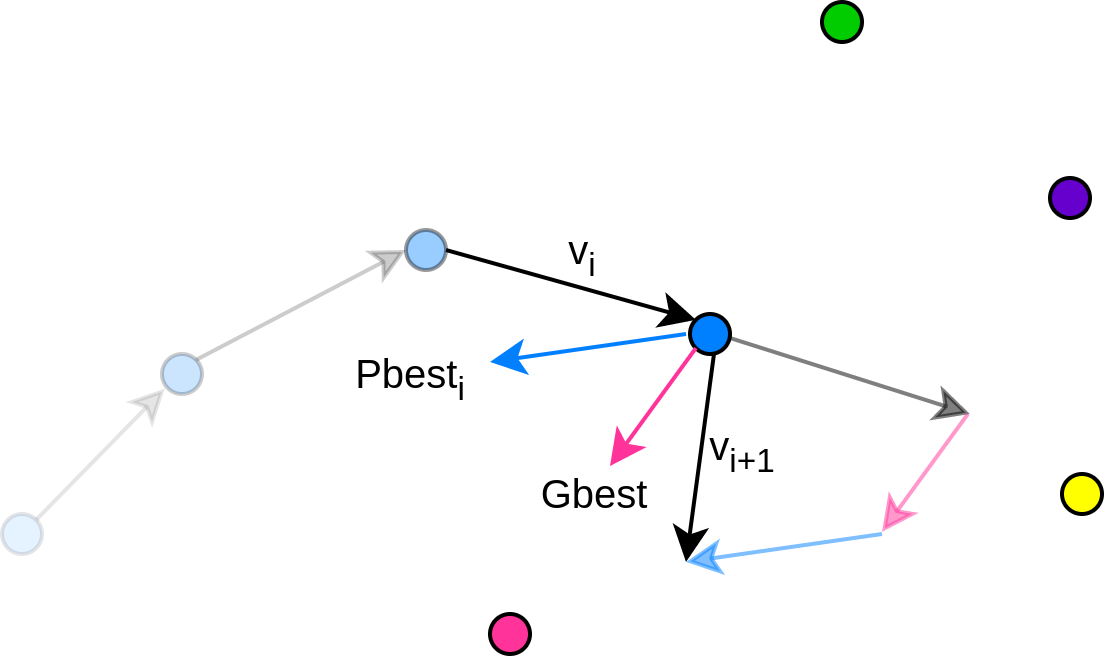
\includegraphics[width=0.7\textwidth]{img/PSO.png}
    \end{center}

    \column{0.5\textwidth}
      Particle Swarm Optimization\bigskip

      \begin{algorithmic}[1]
        \Require $P \in \mathbb{R}^{d\times p}$ (Initial Population)
        \Require $V \in \mathbb{R}^{d\times p}$ (Speed Vector)
        \While{{\bf not} terminate condition}
          \State Pbest $\gets P$, Gbest $\gets$ best($P$)
          \For{$i: 0 \to p$}
          \State $V_i = V_i + w_p*\text{Pbest}_i, w_g*\text{Gbest}$
          \State $P_i = P_i + V_i$
          \State Update Pbest$_i$
          \EndFor
          \State Update Gbest
        \EndWhile
        \State {\bf Output} best $x \in P$
      \end{algorithmic}
  \end{columns}
\end{frame}

\begin{frame}{Different Algorithms, Different Ideas}
  \begin{itemize}
    \item Exploration vs Exploitation;
    \item Parallel Search vs Collaborative Search;
    \item Sequential Search vs Sampling;
    \item Escaping Local Optima;
    \item Niching;
    \item Exploiting Domain Knowledge
  \end{itemize}
  \vfill

  There are many ideas to explore, and they can guide the creation of new algorithms;
\end{frame}


\section{The Rise of the Metaphors}
\begin{frame}
  \begin{center}
  {\large{\bf
  Part II\\
  The Rise of the Metaphors
  }}
  \end{center}
\end{frame}

\subsection{The Birds and the Bees}
\begin{frame}{The Birds and the Bees}
  \begin{block}{Artificial Bee Colony (Karaboga and Dervis, 2005)}
    \begin{itemize}
      \item Population is divided into Worker Bees, Onlooker Bees, Scout Bees
      \item Worker bees find food, evaluate the closest nectar, and \alert{dances}
      \item Onlooker bees observe the dance and go to the closest source
      \item Scout bees replace abandoned food sources with new sources
    \end{itemize}
  \end{block}
  \begin{block}{Cuckoo Search (Yang and Deb, 2009)}
    \begin{itemize}
      \item A cuckoo replaces its solution by using Levy Flight;
      \item Choose a random nest and replace it with a new solution;
      \item Abandon a fraction of the \alert{worst nests};
    \end{itemize}
  \end{block}
\end{frame}

\begin{frame}{There is something strange about the birds and the bees}
  The description of "Artificial Bee Colony" and "Cuckoo Search" feels different from the classical algorithms:\medskip

  \begin{itemize}
      \item What does the dance of the bees mean?
      \item The ABC description does not mention that only one dimention is changed at a time;
      \item Are the solutions in CS the birds or the nests?
      \item "Scout bees" and "Abandon nest" do the same thing; Why different names?
      \item The details of the implementations are not explained fully in the papers.
  \end{itemize}\bigskip

  {\bf Metaphor Heuristics}: The metaphor (birds, bees) is more important than the algorithm
\end{frame}

\subsection{Cambrian Explosion}
\begin{frame}{A Cambrian Explosion of Metaphor Heuristics}
  \begin{center}
  \includegraphics<1>[width=1\textwidth]{img/metaphors_0.png}
  \includegraphics<2>[width=1\textwidth]{img/metaphors_1.png}
  \includegraphics<3>[width=1\textwidth]{img/metaphors_2.png}
  \includegraphics<4>[width=1\textwidth]{img/metaphors_3.png}
  \includegraphics<5>[width=1\textwidth]{img/metaphors_4.png}
  \includegraphics<6>[width=1\textwidth]{img/metaphors_5.png}
  \includegraphics<7>[width=1\textwidth]{img/metaphors_6.png}
  \end{center}
\end{frame}

\subsection{Why is this a bad thing?}
\begin{frame}{What is the problem with Metaphor Heuristics?}
  \begin{itemize}
    \item Are there really over 200 ways to create Search Based Optimization algorithms?
    \item And are metaphors the correct way to organize this research?
  \end{itemize}
\end{frame}

\begin{frame}{Problems with Metaphor Heuristics}{Endlessly Reinventing the Wheel}
  \begin{block}{}
  Because Metaphor Metaheuristics hide their details behind complex metaphors, it is difficult to tell what is similar, and what is different between these algorithms.\end{block}\bigskip

  \begin{itemize}
    \item "The amount of soil on the edges of the iteration-best solution is reduced based on the goodness of the solution"
    \item "This population is generated by a first shot explosion producing a number of individuals (shrapnel pieces)"
    \item "In this case the bait helps the Green Heron bird to catch a prey and thus the solution set elements remain constant"
    \item "The selection of two barnades is based on the length of their penises, pl. The selection process mimics the behaviour of barnacles. [It] is done randomly, but it will be restricted to the penis length of the barnacle"
    \item "The objective function was regarded as invariant to the reference frame, something like a transcendental entity in the space time"
  \end{itemize}
\end{frame}

\begin{frame}{Problems with Metaphor Heuristics}{Spamming the literature, and salami science}
  \begin{itemize}
    \item The literature is flooded with algorithms that are identical or very similar;
    \item These papers lack in reproducibility and analysis standards;
    \item People outside of the field can't see the entire literature, and end up picking the flashier names;
    \item Some suspicious activity, such as salami science and citation rings;
  \end{itemize}\bigskip

  \begin{block}{}
  A paper using purely metaphor language with poor scientific standards will often be non-falsifiable;
  \end{block}
\end{frame}

\subsection{Fighting back the flood}
\begin{frame}{Pushback on Metaphor Algorithms}
  Fortunately, in recent years there has been a push back against this kind of practice.\bigskip

  \begin{itemize}
    \item Kenneth Sorsen, 2015: "Metaheuristics, the Metaphor Exposed";
    \item Villalon, Weyland: Analysis of individual popular metaphors;
    \item Many people: "Metaphor-based Metaheuristics, a call for action"\bigskip

    \item Some Journals have updated their policies to reject "Metaphor Heuristics" (Operations Research, Swarm Intelligence, TELO, Journal of Heuristics, and others)
  \end{itemize}\bigskip

  \begin{block}{}
    Still, we ask ourselves: Then, how do we properly create new metaheuristics?
  \end{block}
\end{frame}
%% Papers about this situation

%%%%%%%%%%%%%%%%%%%%%%%%%%%%%%%%%%%%%%%%%%%%%%%%%%%%%%%%%%%%%%%%%%%%%%%%%%%%%%%%
\section{Component-based Evolutionary Algorithms}

\begin{frame}
  \begin{center}
  {\large{\bf
  Part III\\
  Component-Oriented Evolutionary Computation
  }}
  \end{center}
\end{frame}

\subsection{Algoriths from Components}
\begin{frame}{We still want new meta-heuristic optimizers}

  \begin{block}{}
    \begin{center}
      We don't want to create a new algorithm for everything,\\
      but different problems require different strategies.
    \end{center}
  \end{block}

  \begin{block}{Properties of the Fitness Landscape}
    \begin{itemize}
      \item Number of Local Optima;
      \item Multi-modal problems;
      \item Separability of the parameters;
    \end{itemize}
  \end{block}
  \begin{block}{Properties of the Problem Domain}
    \begin{itemize}
      \item Dynamic Problems;
      \item Multi-Objective problems;
      \item Constraints;
    \end{itemize}
  \end{block}\bigskip

  So, we still need to create ``new algorithms'' from time to time. How to do that responsibly?
\end{frame}

\begin{frame}{Mixing and Matching: The Composition Approach}

  Instead of creating a \alert{{\bf NEW ALGORITHM!}}...\\
  \hfill ...how about re-using the knowledge that already exists?\bigskip
  
  Search-Based Optimizers have a common structure:
  \begin{itemize}
    \item Generate solutions;
    \item Test solutions;
    \item Modify solutions;
  \end{itemize}\medskip

  Can we populate this structure with ``tricks'' that were
  discovered in previous algorithms?
  \begin{itemize}
    \item The mutation from Evolutionary Strategies;
    \item The crossover from Genetic Algorithm;
    \item The velocity from PSO;
    \item etc...
  \end{itemize}\bigskip

  \begin{block}{}
    This is the \structure{Compositional Approach} of algorithm design!
  \end{block}
\end{frame}

\begin{frame}{Imagine the Magic!}{Using the Composition Approach for Algorithm Design}
  \begin{center}
    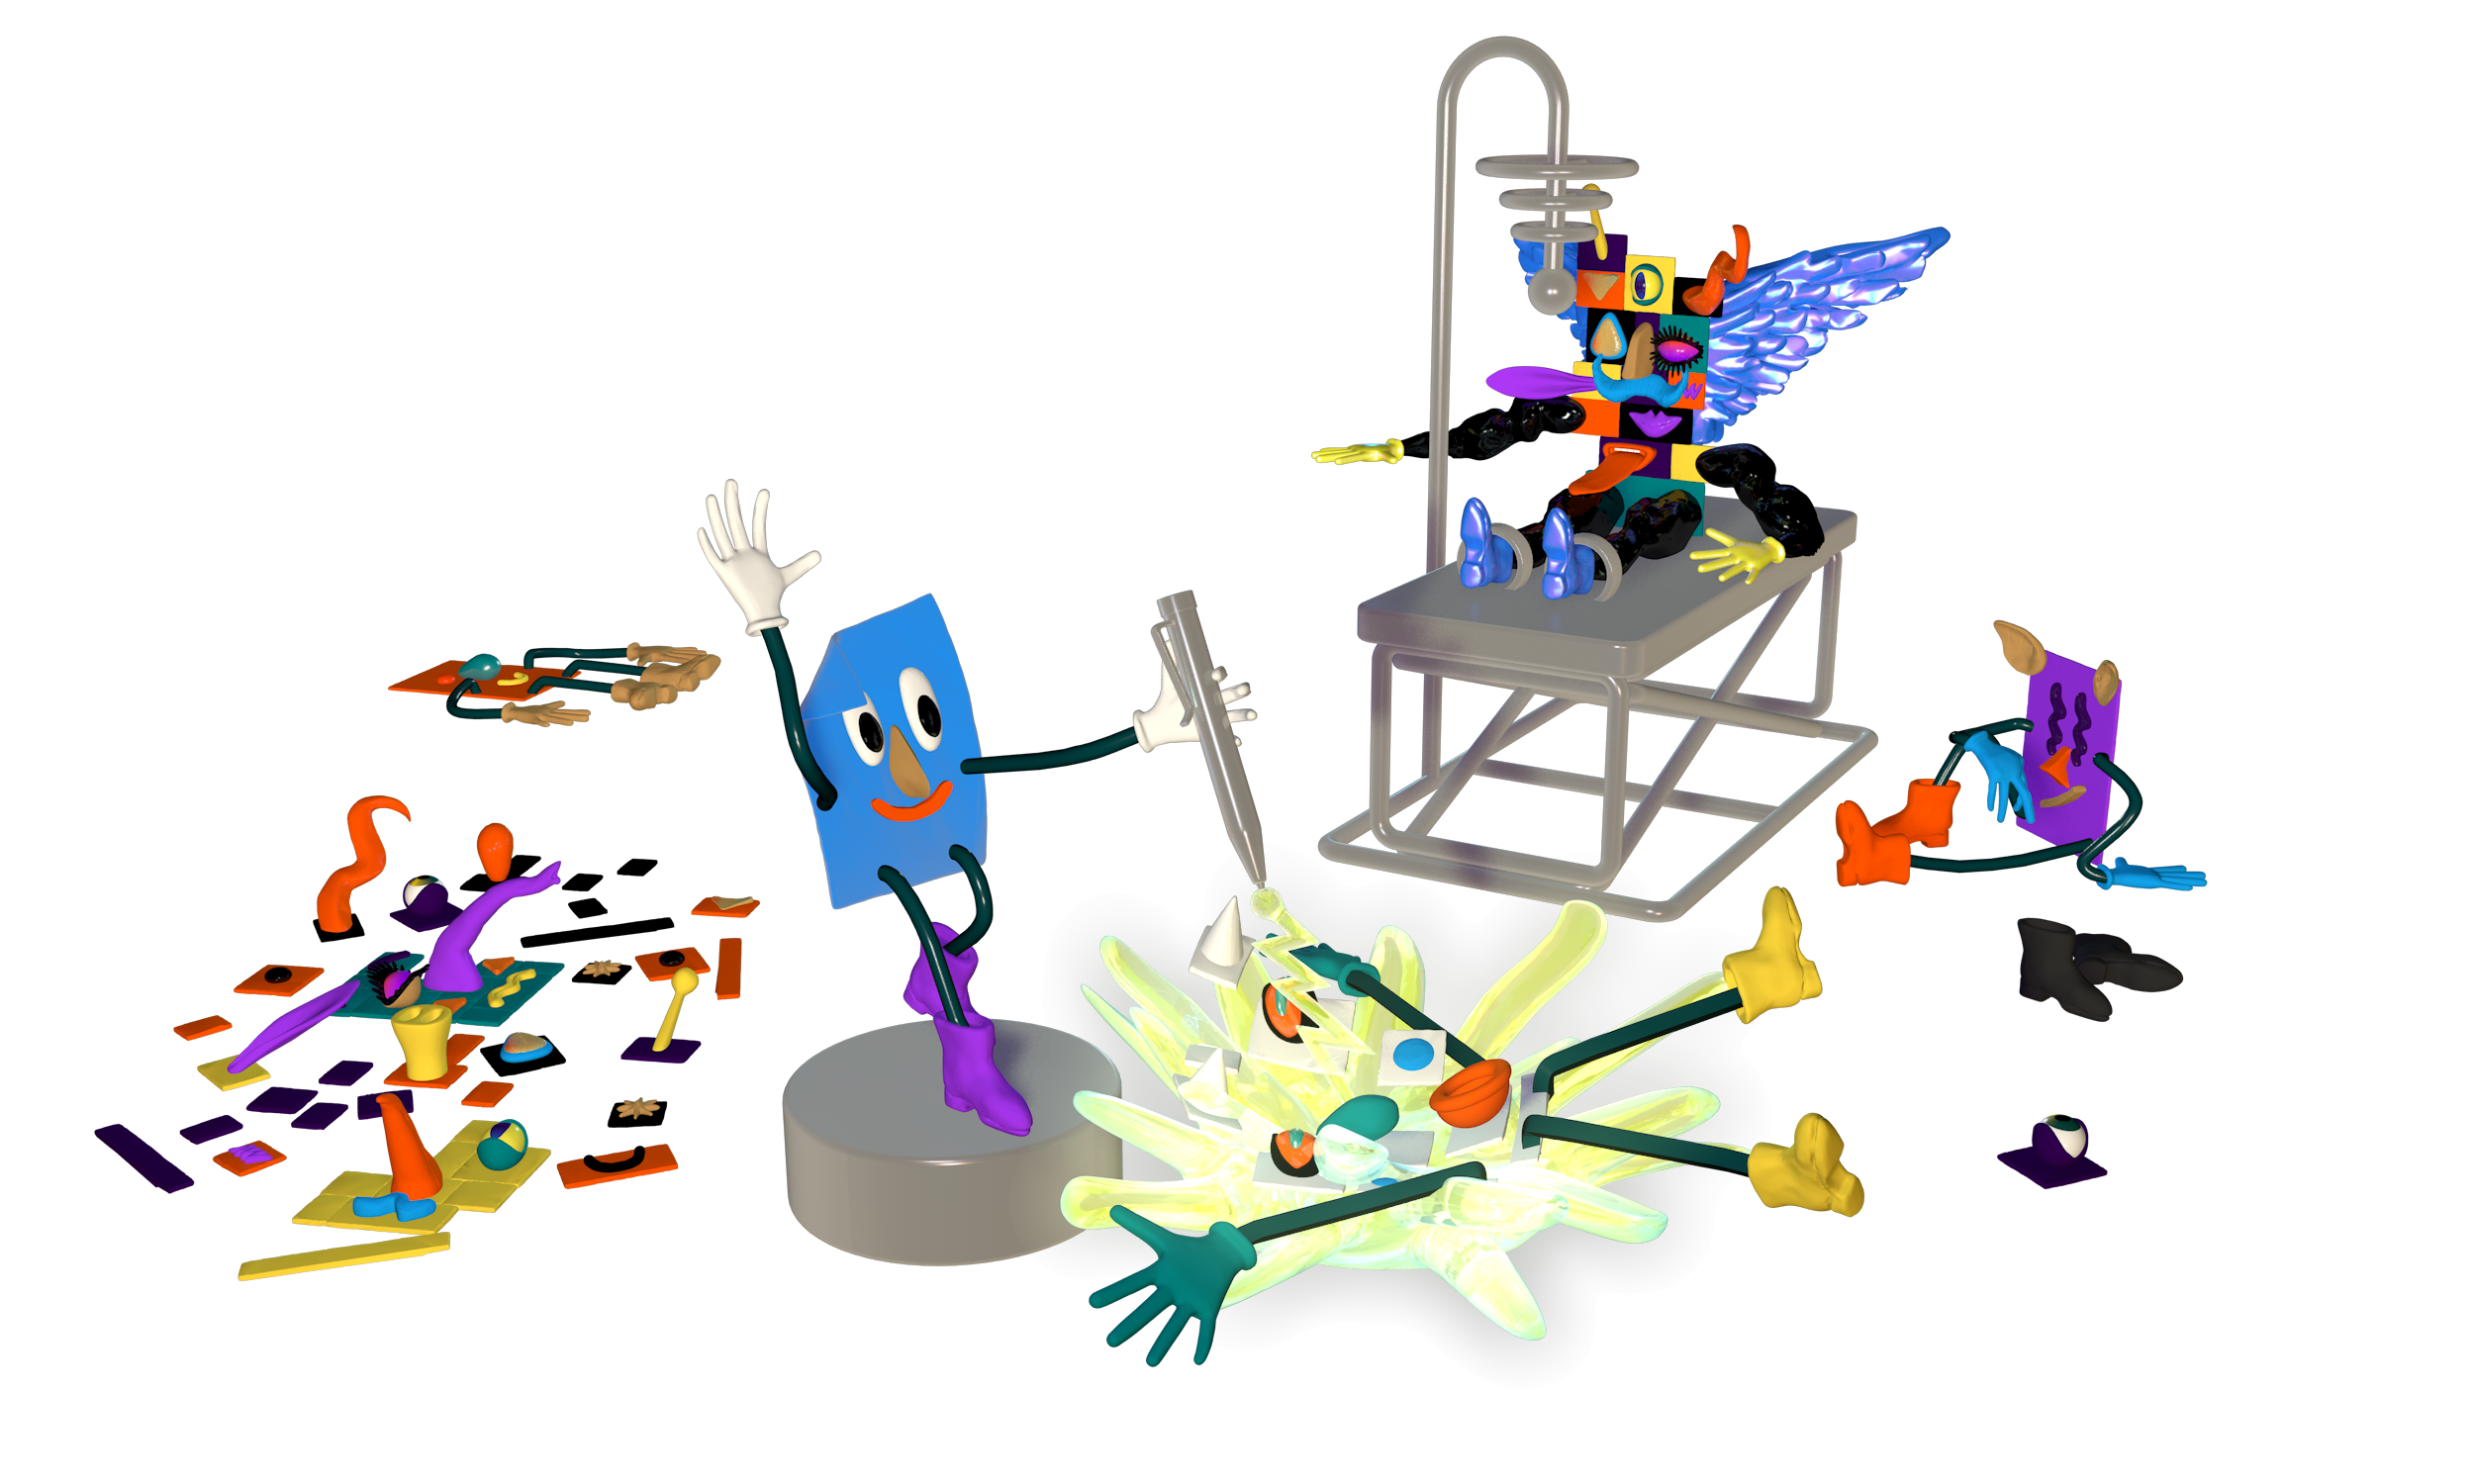
\includegraphics[width=0.85\textwidth]{img/franken_project.png}
  \end{center}
\end{frame}

\begin{frame}{Well... actually it looks more like this}
  \begin{center}
    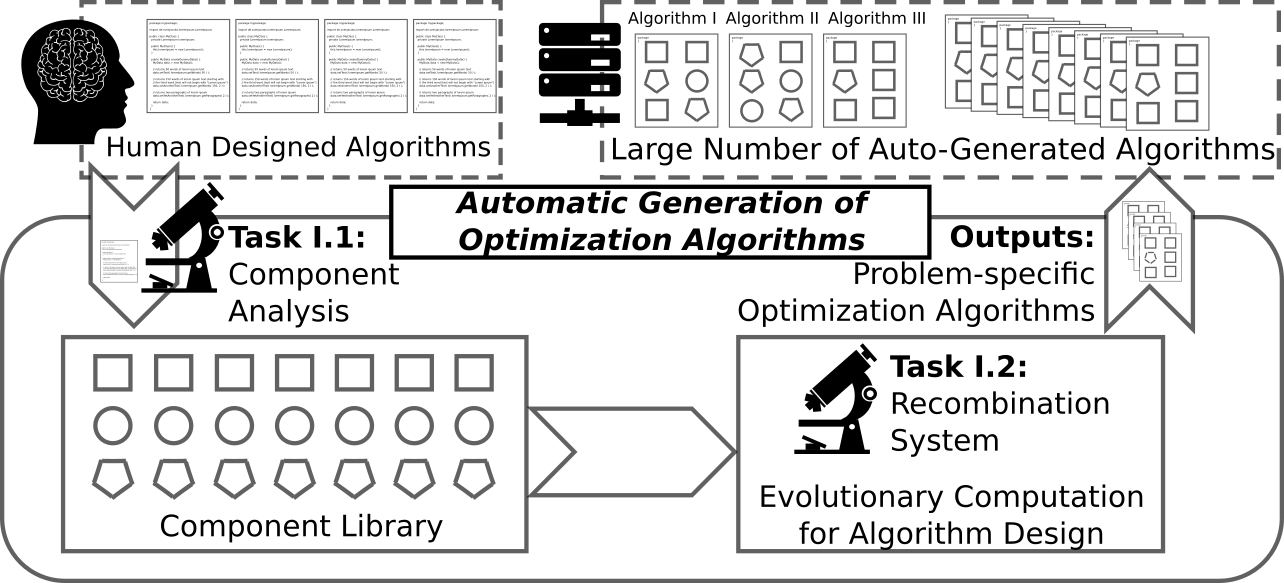
\includegraphics[width=0.8\textwidth]{img/algorithmdesign_project.png}
  \end{center}
  There is a lot to talk about! Today, we will focus on \structure{(1) How to compose the algorithm} and \structure{(2) How to pick the set of components}.
\end{frame}

\subsection{Algorihtm Composition}

\begin{frame}{How to Compose the Algorithm?}{The Parametric Approach}
  One way to automatically compose an optimization algorithm is to
  \structure{Treat the components as {\bf Parameters} of the
    algorithm}.\bigskip

  Then we can use standard algorithm configuration tools (such as
  iRace or SMAC) to choose the best components, given a set of test
  functions.\bigskip

  One early example of this approach is \emph{``Automatic
  Component-Wise Design of Multiobjective Evolutionary Algorithms''}
  (Bezerra et al, 2015), where they set some of the components of an
  MOEA as parameters, and find that they can improve the performance
  of the algorithm by optimizing those.
\end{frame}

\begin{frame}{One big problem in the Composition Approach: the coding!}

  It is fairly difficult to generate a flexible package that can
  compose different algorithms together at the same time.\medskip

  {\bf Why?} Many researchers use non-standard coding patterns (when
  the code is available) or descriptions (when it isn't).\medskip

  It is actually good to do this work, though, as it develop healthy
  programming habits that us researchers don't usually have.

  \begin{columns}
    \column{0.5\textwidth}
    Me and Felipe campelo gave our contribution to this effort by creating {\bf MOEADr},
    a package that implements the MOEA/D algorithm in R, using a component-oriented design.
    \column{0.5\textwidth}
    
\includegraphics[width=0.9\textwidth]{img/xkcd_927_standards.png}
  \end{columns}
\end{frame}
% TODO: Expand on the "good programming habits" part.

% One thing that is really difficult about algorithm composition, is
% that a lot of it is about SOFTWARE ENGINEERING: designing your
% algorithm so that you can switch the components easily, and
% designing the components with a exchangable interface.  It is a lot
% of work for scientists, who are used to write quick and dirty code
% (XGH),

% But it can also be useful to develop healthy programming habits,
% such as testing, etc.  Even if you don't plan to make your
% algorithms configurable to this degree, it can be useful to follow
% these practices to

\subsection{MOEADr}

\begin{frame}{The MOEADr Package}{Campelo and Aranha, 2017--2021}
  The MOEADr is an R package (\structure{You can find it in CRAN!})
  that implements the MOEA/D algorithm, as well as many of its popular
  components.
  \bigskip

  The goal of the package is to allow specific components of the
  MOEA/D framework to be easily added or removed, to facilitate
  automated design.\bigskip

  Let's give a quick look at the main ideas.
\end{frame}

\begin{frame}
  \frametitle{The MOEA/D Framework}

  \begin{block}{}
    The pseudocode below summarizes the MOEA/D algorithm.\\
    The blue comments to the left indicate parts where we can replace components.
  \end{block}
  
  {\scriptsize
      \begin{algorithmic}[1]
        \Require Objective functions $\mathbf{f}(\cdot)$; Constraint
        functions $\mathbf{g}(\cdot)$;
        \Require Component-specific input parameters;    
        \State $t\leftarrow 0$; $run\leftarrow \mbox{TRUE}$
        \State Generate initial population $\mathbf{X}^{(t)}$ by random sampling.\Comment{\structure{Initialization}}
        \State Generate weights $\Lambda$ \Comment{\structure{Decomposition
          strategies}}
        \While{$run$}
        \State Define or update neighborhoods $B$
        \Comment{\structure{Neighborhood assignment strategies}}
        \State Copy incumbent solution set $\mathbf{X}^{(t)}$ into $\mathbf{X}^{\prime~(t)}$
        \For{each variation operator $\mathbf{v} \in \mathcal{V}$}
        \State $\mathbf{X}^{\prime~(t)} \leftarrow v(\mathbf{X}^{\prime~(t)})$
        \Comment{\structure{Variation Stack}}
        \EndFor
        \State Evaluate solutions in $\mathbf{X}^{(t)}$ and
        $\mathbf{X}^{\prime~(t)}$ \Comment{\structure{Aggregation functions
          and Constraint handling}}
        \State Define next population $\mathbf{X}^{(t+1)}$\Comment{\structure{Update
          strategies}}
        \State Update $run$ flag; $t\leftarrow t+1$ \Comment{\structure{Stop criteria}}
        \EndWhile
        \vspace{.10cm}
        \State {\bf return}
        $\mathbf{X^{(t)}};~\mathbf{f}\left(\mathbf{X}^{(t)}\right)$
      \end{algorithmic}
  }
\end{frame}

\begin{frame}
  \frametitle{MOEA/D Component Classes}

  \begin{block}{}
    To facilitate the component design, we separate the MOEA/D
    component in three classes, and each class had a common structure.
  \end{block}\bigskip

  {\smaller
  \begin{columns}
    \column{0.4\textwidth}
      \begin{itemize}
      \item Decomposition Strategy
      \item Aggregation Function
      \item Objective Scaling Strategy
      \item \alert{Neighborhood Assignment Strategy}
      \item \alert{Variation Operator Set}
      \item \alert{Update Strategy}
      \item \structure{Constraint Handling}
      \item \structure{Termination Criteria}
      \end{itemize}
      
      \column{0.6\textwidth}
      \begin{alert}{}
        The components in black deal with the decomposition of a
        multi-objective problem into several single-objective
        problems. This is the main characteristic of MOEA/D.

      \end{alert}
      \begin{alertblock}{}
        The components in red perform the modification and update of
        solutions, based on their fitness values. There is a large
        variety of designs here, including operators from other
        algorithms.  To deal with this variety, we designed a
        \structure{Variation Stack}.
      \end{alertblock}
      \begin{exampleblock}{}
        The components in Blue handle methods to modify the result of
        the fitness evaluation. Although this is usually problem
        specific, there are some common ways to handle constraints.
      \end{exampleblock}
  \end{columns}
  }
\end{frame}


\begin{frame}
  \frametitle{Components Implemented by the MOEADr Package (v1.0.1)}

  {\scriptsize
    \begin{center}
      
\renewcommand{\arraystretch}{1.4}

  \begin{tabular}{|c|c|c|}
    \hline
    \textbf{Component Class} & \textbf{Name} & \textbf{User Parameters} \\
    \hline
    \multirow{3}{*}{Decomposition Method}& 
	SLD & $h\in\mathbb{Z}_{>0}$\\
	\cline{2-3}
    & MSLD & $\mathbf{h}\in\mathbb{Z}^{K}_{>0}$; $\tau\in\left(0,1\right]^{K}$\\
    \cline{2-3}
    & Uniform& $N\in\mathbb{Z}_{>0}$\\
    \hline
    \multirow{5}{*}{Scalar Aggregation Function}& 
    WS& -- \\
    \cline{2-3}
    & WT& -- \\
    \cline{2-3}
    & AWT& -- \\
    \cline{2-3}
    & PBI& $\theta^{pbi}\in\mathbb{R}_{>0}$ \\
    \cline{2-3}
    & iPBI& $\theta^{ipbi}\in\mathbb{R}_{>0}$ \\
    \hline
Objective Scaling& 
	-- & $type\in\left\{none;~simple\right\}$ \\
    \hline
\multirow{2}{*}{Neighborhood Assignment}& 
	\multirow{2}{*}{--} & $type\in\left\{by~\lambda_i;~by~\mathbf{x}_i^{(t)} \right\}$ \\
	\cline{3-3}
	& & $\delta_p\in\left[0,1\right]$ \\
        \hline
        
    \end{tabular} 

    \end{center}
  }
\end{frame}

\begin{frame}
  \frametitle{Components Implemented by the MOEADr Package (v1.0.1)}

  {\scriptsize
    \begin{center}
      
\renewcommand{\arraystretch}{1.4}

  \begin{tabular}{|c|c|c|}
    \hline
    \textbf{Component Class} & \textbf{Name} & \textbf{User Parameters} \\
    \hline
\multirow{9}{*}{Variation Operators}& 
SBX recombination & $\eta_{\mathtt{X}}\in\mathbb{R}_{>0}$; $p_{\mathtt{X}}\in\left[0,1\right]$ \\
	\cline{2-3}
	& Polynomial mutation & $\eta_{\mathtt{M}}\in\mathbb{R}_{>0}$; $p_{\mathtt{M}}\in\left[0,1\right]$\\
	\cline{2-3}
	& \multirow{2}{*}{Differential mutation}& $\phi\in\mathbb{R}_{>0}$ \\
	& & $basis \in\left\{rand;~mean;~wgi\right\}$\\
	\cline{2-3}
	& Binomial recombination&$\rho\in\left[0,1\right]$ \\
	\cline{2-3}
	& Truncation& --\\
	\cline{2-3}
	& \multirow{3}{*}{Local search} &$type \in\left\{tpqa;~dvls\right\}$ \\
	& & $\tau_{ls}\in\mathbb{Z}_{>0}$; $\gamma_{ls}\in\left[0,1\right]$ \\
	& & $\epsilon\in\mathbb{R}_{>0}$ (if $type = tpqa$) \\
    \hline
\multirow{3}{*}{Update Strategy}& 
	Standard & --\\
	\cline{2-3}
	& Restricted & $nr\in\mathbb{Z}_{>0}$\\
	\cline{2-3}
	& Best &$nr\in\mathbb{Z}_{>0}$; $T_r\in\mathbb{Z}_{>0}$ \\
    \hline
    \end{tabular} 

    \end{center}
  }
\end{frame}

\begin{frame}
  \frametitle{Components Implemented by the MOEADr Package (v1.0.1)}

  {\scriptsize
    \begin{center}
      
\renewcommand{\arraystretch}{1.4}

  \begin{tabular}{|c|c|c|}
    \hline
    \textbf{Component Class} & \textbf{Name} & \textbf{User Parameters} \\
    \hline
\multirow{3}{*}{Constraint Handling}&
	Penalty functions& $\beta_v\in\mathbb{R}_{>0}$ \\
	\cline{2-3}
	& \multirow{2}{*}{VBR}& $type \in \left\{ts;~sr;~vt\right\}$ \\
	& & $p_f\in\left[0,1\right]$ (if $type = sr$) \\
	\hline
\multirow{3}{*}{Termination Criteria}&
	Evaluations& $max_{eval}\in\mathbb{Z}_{>0}$ \\
	\cline{2-3}
	& Iterations& $max_{iter}\in\mathbb{Z}_{>0}$ \\
	\cline{2-3}
	& Time& $max_{time}\in\mathbb{R}_{>0}$ \\
    \hline
    \end{tabular} 

    \end{center}

    \vspace{1cm}
  }
    We hope to include new components soon!

\end{frame}

\subsection{Grammatical Evolution}

\begin{frame}{Genetic Programming Approach}
  Another way to to approach the automatic design of algorithms is
  through \structure{Genetic Programming}.\bigskip

  Genetic programming is an amazing technique that uses evolution for
  the design and improvements of programs. So the idea is:\\
  \structure{Can we use Genetic Programming for the design of meta
    heuristics?}\bigskip

  \begin{columns}
    \column{0.5\textwidth}
    There is a big problem though:\medskip

    Genetic programming still has difficulty with programs involving
    loops and complex data structures... \structure{what can we do?}
    \column{0.5\textwidth}
    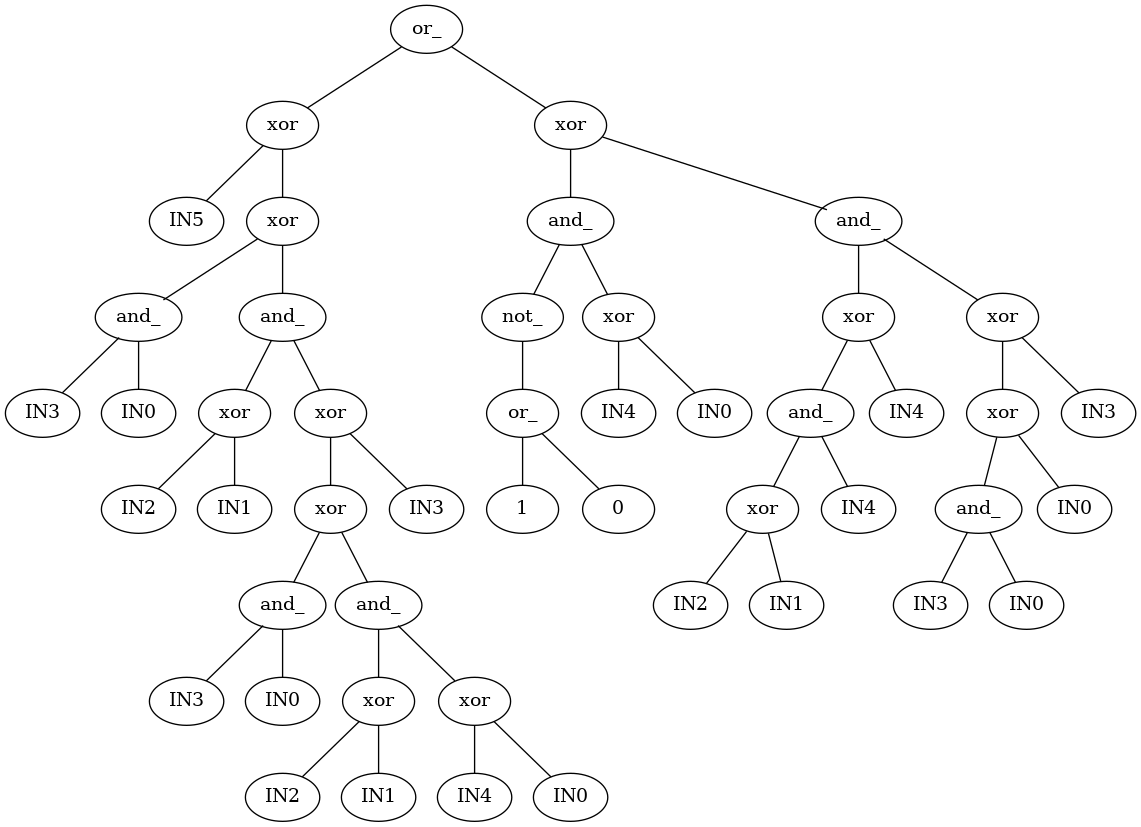
\includegraphics[width=0.7\textwidth]{img/GP_tree_big.png}
  \end{columns}
\end{frame}

\begin{frame}{Using Grammatical Evolution to generate meta-heuristics}{Bogdanova, Pereira, Aranha, 2019}
  \begin{columns}
    \column{0.6\textwidth}

    We used \structure{Grammatical Evolution (GE)} to automatically
    generate Swarm-like (DE, PSO, etc) heuristics.\bigskip

    Genetic Evolution uses a \emph{formal grammar} to defines the general
    structure of a SWARM heuristic. This formal grammar can express:
    \begin{itemize}
      \item Commands;
      \item Loops and Recursion;
      \item Conditions / Stop conditions;
    \end{itemize}\medskip

    So it is more powerful than just treating components as
    parameters.
    \column{0.4\textwidth}
    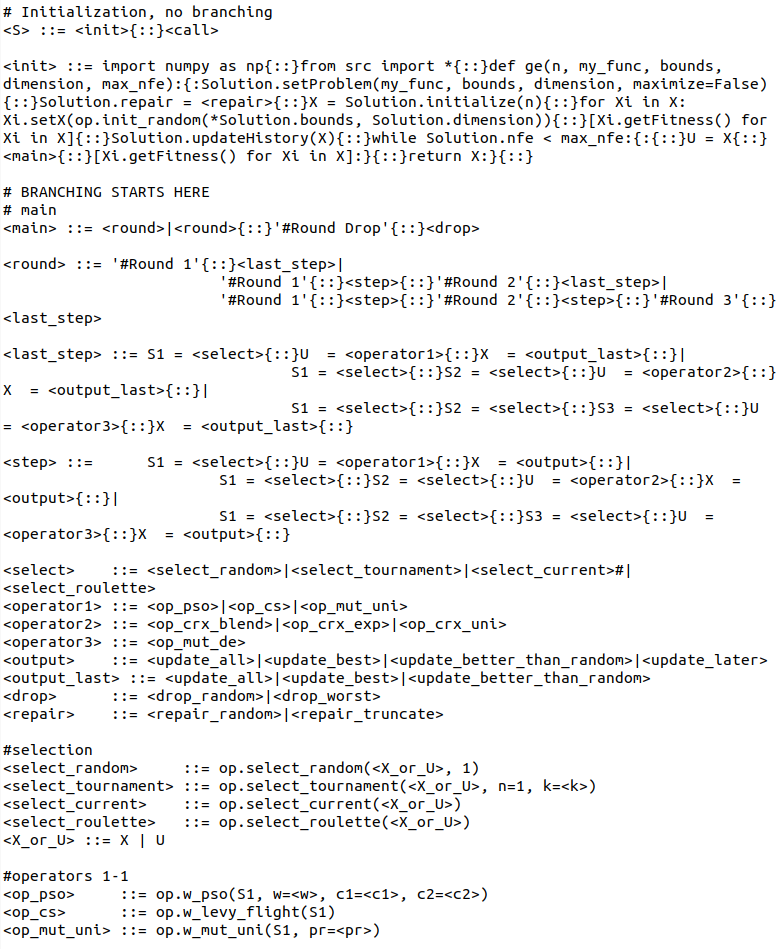
\includegraphics[width=0.9\textwidth]{img/GE_setup.png}
  \end{columns}
\end{frame}

\begin{frame}[fragile]{Example of a Formal Grammar}
  \begin{columns}
    \column{0.6\textwidth}
    Grammar:
\begin{verbatim}
S := A| A * A
A := A + A | A - A | B
B := X | Y | B * B
\end{verbatim}

Examples of instances of this Grammar:
\begin{itemize}
 \item Y
 \item X + X - Y
 \item (Y - XY) + (X - (Y + Y))
\end{itemize}\bigskip

This example is very simple, but I hope it shows that grammars can
generate complex combinations, and complex programs.
    
    \column{0.4\textwidth}
    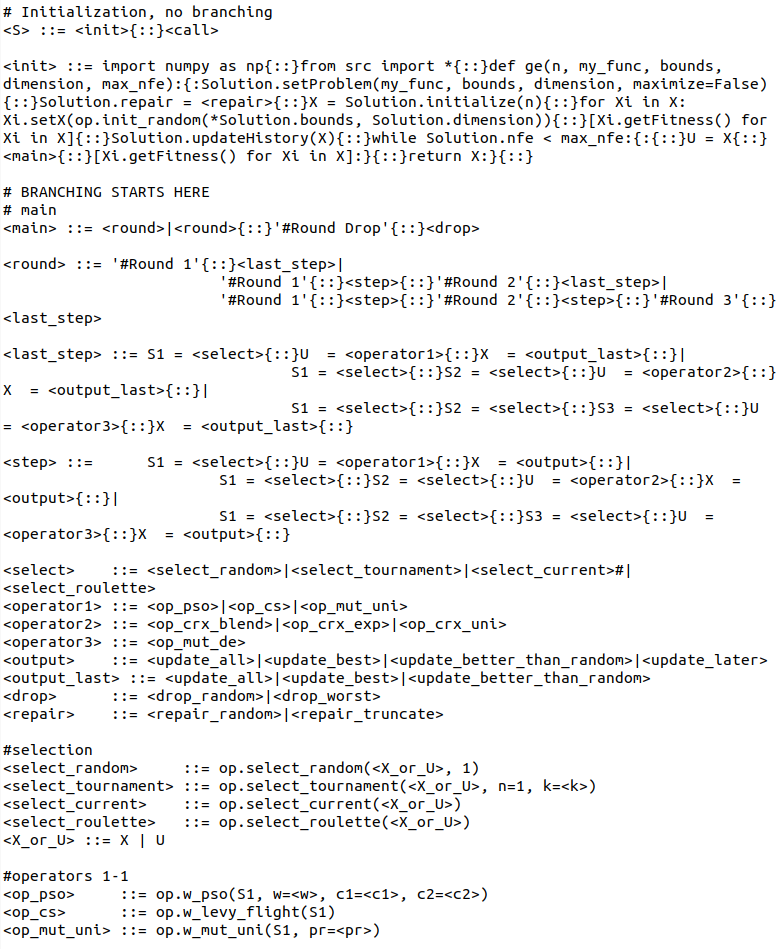
\includegraphics[width=0.9\textwidth]{img/GE_setup.png}
  \end{columns}
\end{frame}


\begin{frame}{What did we achieve with Grammatical Evolution?}
  \structure{Things that worked:}
  \begin{itemize}
  \item We found a good grammar and components that could generate popular swarm meta-heuristics;
  \item Using this grammar, GE could also generate ``crazy'' algorithms;
  \item The algorithms performed well on simple benchmarks;
  \end{itemize}
  \bigskip

  \alert{Things that did not work:}
  \begin{itemize}
  \item Grammatical evolution is {\bf very} slow...
  \item Fitness is difficult: Too hard, and algorithms don't generate; Too easy, and algorithms don't evolve;
  \item How to choose components for more general algorithms?
  \end{itemize}
\end{frame}

% TODO: fit the talk about difficulty schedule

\subsection{Selecting Components}
\begin{frame}{How to select components?}
  \begin{columns}
    \column{0.7\textwidth}
    The two approaches that we described below rely on using a {\bf
      common framework}, and selecting components for building this
    framework.\bigskip

    ... But how do we select which components to add to these approaches?
    \column{0.3\textwidth}
    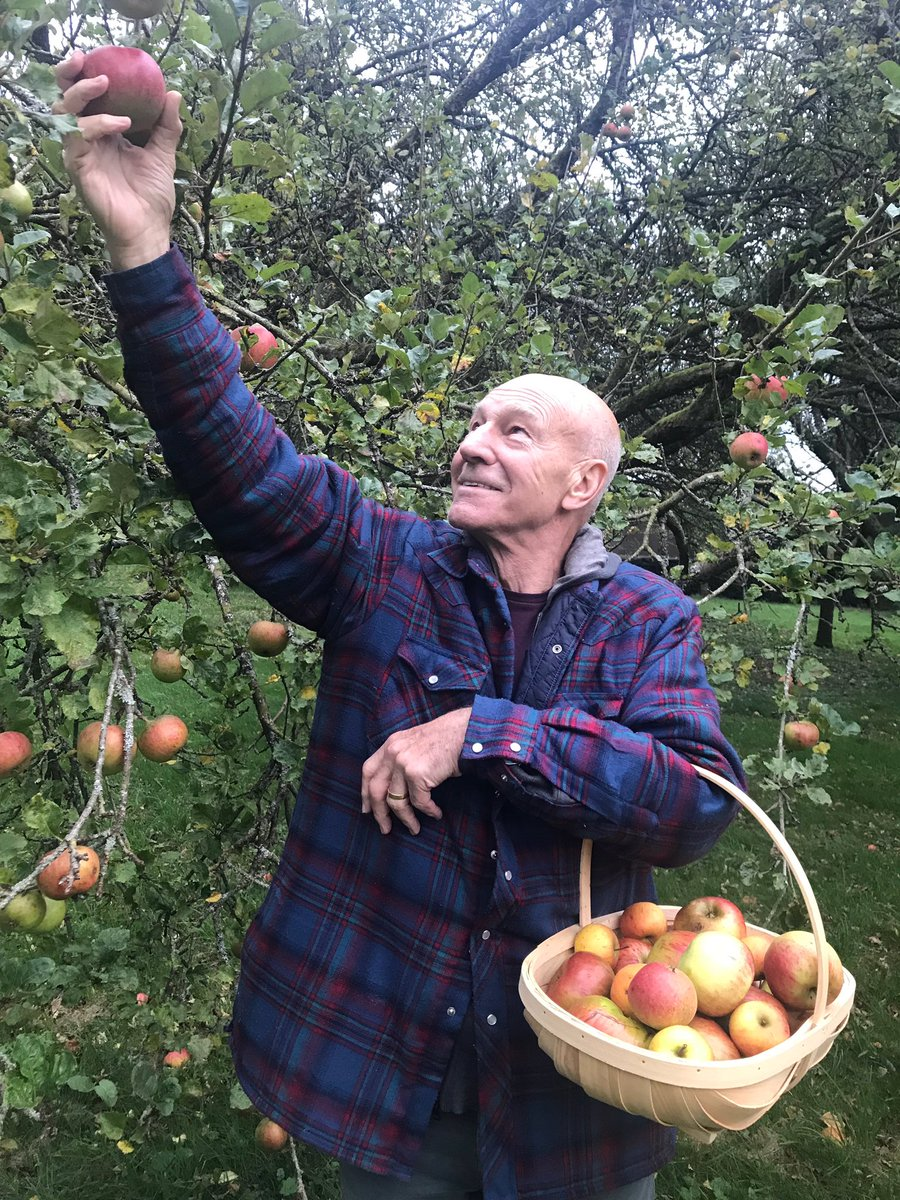
\includegraphics[width=0.9\textwidth]{img/selecting_components.jpg}
  \end{columns}
\end{frame}

%% Selecting Components
\begin{frame}{Selecting components from algorithm analysis}

  The obvious way to select components is to \structure{study many
    algorihtms and extract promising techniques from them}.\bigskip

  But this is not a very good answer, there are many open questions!
  \begin{itemize}
  \item There are too many algorithms to study, and some of them are too similar;
  \item Which algorithms are more or less efficient?
  \item If the algorithms use different languages, how do we compare them?
  \end{itemize}
\end{frame}


\begin{frame}{Algorithm Similarity Measures}
  This leads us to the question of...
  \begin{block}{}
    \begin{center}
      How do we measure the similarity of two Search-Based Optimization Algorithms?
    \end{center}
  \end{block}\bigskip

  Why do we want to measure the similarity of algorithms?
  \begin{itemize}
  \item Identify groups of algorithms with useful components;
  \item Create an ensemble of algorithms with different characteristics;
  \item Select new algorithms when old ones are not performing well
    against a problem;
  \end{itemize}
\end{frame}

\begin{frame}{Literature: Manual Similarity Analysis}
  Earlier work analyzed algorithms manually to find patterns, and
  classify them following those patterns:\bigskip

  \begin{itemize}
  \item {\bf Lones, 2014}: Define strategies for SBO's, and classify
    algorithms by these strategies. For example,
    \structure{Directional Search}.
  \item {\bf Lones, 2020}: Continues the above work by designing a
    standardised description of strategies and operators based on PSO.
  \item {\bf Armas, 2021}: Defines a pool template (list of
    components) for algorithms, and measure similarity by the number
    of shared components in the template.
  \end{itemize}
\end{frame}

\begin{frame}{Automated Similarity Analysis}{Pereira and Aranha, 2022 (BIOMA)}
  Recently, we explored the automation of some of the work done by Lones and Armas.
  \begin{itemize}
    \item There are just too many algorithms in the literature to
      compare manually (and new ones are proposed all the time!)
    \item If we are automating the composition of algorithms, it makes
      sense to automate the similarity measure too!
  \end{itemize}\bigskip

  But what criteria do we use to compare algorithms?
  \begin{itemize}
  \item It is hard to automatically measure ``algorithmic patterns'';
    % We could do code analysis, maybe, but is it possible to compare
    % two algorithms based only on their code trace? No idea.
  \item On the other hand, pure performance could hide differences;
    % Different performance in different functions/problems. Different
    % metrics: machine load, convergence speed, diversity, robustness,
    % other performance metrics
  \item Also, how do we measure the effect of changes in parameters?
    % When parameters change, the performance of algorithms might
    % change. Some algorithms might be more sensitive to parameters
    % than others, and we want to take that into account when
    % measuring the similarity of algorithms.
  \end{itemize}
\end{frame}

\begin{frame}{Automated Similarity Analysis}
  {Our current approach: Clustering Algorithm Instances (Pereira and Aranha, 2022)}
  
  % cluster - based method: Generate several instances for each
  % algorithm. Obtain "features" by running these instances on
  % problems with different known characteristics. Use these features
  % to cluster the algorithms, and analysing the clusters that are
  % formed.

  \begin{columns}
    \column{0.63\textwidth}
    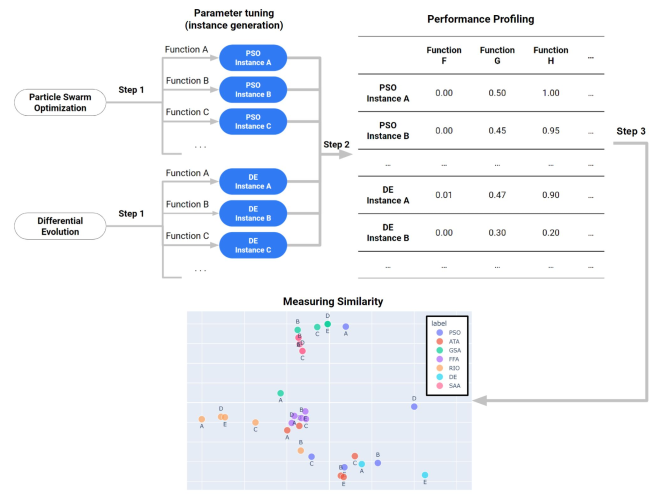
\includegraphics[width=1\textwidth]{img/algo_cluster_flow.png}
    \column{0.37\textwidth}
           {\bf Key Idea:}
           \structure{Cluster-based method}
    \begin{enumerate}
    \item Generate several instances of each algorithm by varying their parameters;
    \item Obtain ``features'' by profiling these instances on
      carefully selected benchmark problems;
    \item Cluster the algorithm instances based on the features, and analyze the result;
    \end{enumerate}    
  \end{columns}
\end{frame}

\begin{frame}{Automated Similarity Analysis}{New Idea: Performance Profile}

  \structure{Performance Profile}: Used to characterize an algorithm
  (or algorithmic instance).

  Composed of an array with the performance value on a set of benchmark problems.\bigskip

  \structure{Performance Similarity}: Measure to compare two
  algorithms based on their Performance Profile.

  \begin{eqnarray*}
    PS(A,B) &=& \sqrt{\sum^n_{i=1}(e^A_i - e^B_i)^2}\\
    e^X_i&=&log_{10}(f^X\text{value}_i - f\text{opt}_i)
  \end{eqnarray*}

  \begin{itemize}
  \item $f^X\text{value}_i$: the value obtained by algorithm $X$ on problem $i$.\\
  \item $f\text{opt}_i$: the optimum of problem $i$.\\
  \end{itemize}

\end{frame}

\begin{frame}{Some Results}
  \begin{itemize}
  \item PSO instances clustered poorly, FFA instances clustered well:
    \begin{itemize}
    \item This indicates parameter dependence?
    \end{itemize}
  \item Clustering limited by positive scores (low difficulty benchmarks?)
  \item Silhouette score used to evaluate cluter quality: Not a good metric here.
  \end{itemize}

  \begin{center}
    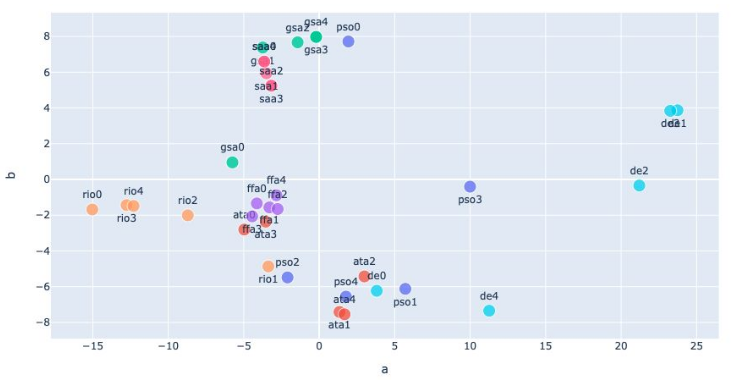
\includegraphics[width=0.6\textwidth]{img/jair_cluster_result.png}
  \end{center}
\end{frame}

\begin{frame}{This research generates several interesting ``Open Questions''}
  \begin{itemize}
  \item {\bf Which metrics to use as attributes?}\\
    What are good metrics to clearly show the difference between
    algorithms, for a set of benchmarks?

  \item {\bf How to select the functions for the Performance Profile?}\\
    Alternatively, what are good sets of benchmarks that show the
    difference between algorithms clearly?

  \item {\bf Can we use this to evaluate the quality of benchmarks?}\\
    We create benchmark based on our theoretical knowledge about how
    blackbox problems should operate. But is this correct? Can we
    confirm that knowledge through this analysis?


  \item {\bf Maybe automatically generate good benchmarks using this
    and GP?}\\
    Can we generate benchmark functions that maximize the distance
    between algorithms? Or maybe adversarially generate benchmarks
    that cause good algorithms to perform poorly?
  \end{itemize}
\end{frame}

%\subsection{Component Analysis}
%\begin{frame}{Component Analysis}
%  % TODO
%  Work of Yuri
%\end{frame}

%%%%%%%%%%%%%%%%%%%%%%%%%%%%%%%%%%%%%%%%%%%%%%%%%%%%%%%%%%%%%%%%%%%%%%%%%%%%%%%%%%
\section{Final Thoughts}

\begin{frame}
  \begin{center}
  {\large{\bf
  Part IV\\
  The End
  }}
  \end{center}
\end{frame}

\begin{frame}{Final Thoughts}
  \begin{itemize}
  \item Evolutionary Computation has been used, with success, to solve
    a variety of Optimization Problems;\medskip

  \item Because there are many different problems, we want to design
    specific algorithms for each of them;\medskip

  \item However, careless development of new algorithms can fragment
    our knowledge base;\medskip

  \item A more organized approach is \structure{component oriented
    design}, which focuses on variations of algorithms using well
    known base frameworks;\medskip

  \item There are many challenges in the research and development of
    component-oriented EA, but it is a very fun challenge for people
    interested in programming.\medskip

  \item There is still a lot of work to do!
  \end{itemize}
\end{frame}

\begin{frame}
  \begin{center}
  {\large{\bf
    Thank you for listening!
  }}
  \end{center}

  % To know more:
  % \begin{itemize}
  %   \item Introduction to Evolutionary Computation: % Springer book?
  %   \item The Metaphor Craze: % Soresen paper, Campelo's LIFELIKE talk?
  %   \item Algorithm Composition: % Some recent conference session?
  %   \item Automatic Algorithm Analysis: % Jair's papers?
  % \end{itemize}
\end{frame}

\end{document}
